%!TEX TS-program = xelatex 
%!TEX encoding = UTF-8 Unicode 
%!TEX root = ../DESpecs.tex


%\section*{XeTeX test}
%\newfontfamily{\A}{Geeza Pro} 
%\newfontfamily{\H}[Scale=0.9]{Lucida Grande} 
%\newfontfamily{\J}[Scale=0.85]{Osaka} 
%XeTeX reconciles LaTeX with Unicode.
%German characters: äöüß, 
%formulas: $x^2 \to \sin \frac{\sqrt{2}}{2}$. 
%Here are some multilingual Unicode fonts: 
%this is Arabic text: {\A السلام عليكم}, 
%this is Hebrew: {\H שלום}, 
%and here's some Japanese: {\J 今日は}. 

%\section*{General Specifications}
%...
 
\section{Structural Markup}

\subsection{Pages and Page numbers}

\begin{mainrule}
Page breaks are tagged by <page>. (Rather than <pb> ? Or <page/> instead? What is a “milestone” tag??) If the page has a page number, such as 34 or iii or VI, it is written thus: <page ... >. A blank line may be inserted before the <page> tag. 
\end{mainrule}

\begin{example}

\begin{type}
\begin{tabular}{l}
text line \\
text line \\
\\
<page 34> \\
text line \\
text line 
\end{tabular}
\end{type}

muh

\end{example}

(Do we need an ECHO image, or does a schematic example suffice?)

\subsection{Headers}

(from the archimedes specs)

<h>text</h>

all headings are tagged in the same way. (will the font size be ignored?)

\subsection{Paragraphs} 

Paragraphs should be marked by <p> at the beginning and </p> at the end. Example: ... (Again: ECHO image or schematic example?)


See also the example in section \ref{Structural markup general example}.

\subsection{Columns}

Use <col> and </col> to tag columns.


Sometimes one column fills the whole width of the page. Still treat it as a column. (leave out this rule because the specs become too long?)

\subsection{Sentences}

Sentences will not be tagged. (Leave out this non-instruction?)

\subsection{Line breaks}

Line breaks will be typed as such, without additional tags. A word separation mark is typed as hyphen. 

Do not insert a space at the end. (The idea is that without this rule the results of two different typists will invariably differ. On the other hand, this is easy to normalise in the post-processing stage. How does the Chines firm decide if the results of two typists are the same? A third person compares it and either finds or does not find ay differences? Then this rule would be superfluous and would in fact hinder the workflow.)

(is singular "a word separation mark" more clear than plural?)

Example: 

\includegraphics[scale=0.5]{bsp_paragraphshort_euclidlat_9} 

\begin{type}
\begin{tabular}{l}
RENSIS CLARISSIMI PHILOSOPHI, MATHEMA- \\
ticorum facilè principis, primùm ex Campano, deinde ex Theone Grӕco \\
cõmentatore, interprete Bartholomӕo Zamberto Veneto, 
\end{tabular}
\end{type}

(Is it asked too much to recognise word separation marks? But then, how should one type an “equality sign in inverse italics”?)


\subsection{Blank lines} 

Do not insert blank lines. (Or: You can insert blank lines? An explicit "do not insert" rule will probably be ignored anyway?

\subsection{Marginal notes}

A marginal note should be typed in separate lines, after the line of the main text where it occurs (or: after the line it is the closest to). Use the <m> and </m> tag. 

(The post-processing effort of adjusting marginal notes is small compared to the effort of typing them, so it does not make sense to make this rule too precise or to have complicated rule variations for marginal notes to the left and to the right of the main text. Or does it make sense to say something like: a blank line before/after the marginal note indicates that the note ist to hte right/left of the main text? Or <marginal left>, <marginal right> ? But again: How are the results of two typists compared? Do they know that having the marginal note one line above or below doesn't matter?)

Example: image left marginal note, image right marginal note.

\includegraphics[scale=0.9]{bsp_marginalnote_coimbricenses_232} 

\begin{tabular}{l}
main text \\
<marginal>marginal text\\
marginal text \\
marginal text</marginal> \\
main text \\
\end{tabular}

Would <m> be better than <marginal>? Do they speak English or is an English word just longer to type for them?

Handwritten marginal notes should \emph{not} be typed.

(Do we need an example here?)

\includegraphics[scale=0.35]{bsp_handmargin2_benedetti_174} 

\subsection{Footnotes}

A footnote should be typed where it occurs, but in separate lines. Use the <fn> and </fn> tag. Ignore the footnote symbol in the main text. Type it in the <fn> tag, but ignore the superscript.

Example [image]: this word$^1$ has a footnote

\begin{tabular}{l}
this word \\
<fn 1> footnote text \\
footnote text</fn> \\
has a footnote \\
\end{tabular}

Alternative:

\begin{tabular}{l}
this word 1 has a footnote \\
<fn 1> footnote text \\
footnote text</fn> \\
\end{tabular}

Another alternative: Ignore the semantics of the footnote, write the footnote symbol in superscript in the main text, type in the footnote where it occurs on the text?

Archimedes (note: <n> vs. <fn> !?)

\begin{tabular}{l}
this word...<n 1> has a footnote \\
<fn 1> footnote text \\
footnote text</fn> \\
\end{tabular}

(what are common footnote symbols at this that time? Do we need to provide a list with <01> replacements for weird symbols?)

\subsection{Figures}

(Follow the workflow for the mechanics project? <p>text<figure/></p> ??)

(Does it make sense to make them distinguish between sheer ornaments and figures? Would be easy to distinguish at the post-processing stage.)

Where the figure occurs, Put a <figure> tag in a separate line.

Example images: between paragraphs, between lines of one paragraph, left/middle/center position and the text is floating around it, between two columns (treat as to the right of the left column)?

\begin{tabular}{l}
text</p> \\
<figure> \\
<p>text \\
\end{tabular}

\begin{tabular}{l}
text \\
<figure> \\
text \\
\end{tabular}

And so on.

\subsection{Tables and lists}

\subsection{Catchwords and Signatures}

Catchwords and signatures at the bottom of the page should not be typed.

Example

\includegraphics[scale=0.35]{bsp_catchwordsignature_benedetti_191} 


\subsection{Unrecognizable characters}

Obscure characters: Chinese firm should make list, e.g. <01> etc., use consistently.

Creases, etc.

General tag “there is a problem”, applicable to characters, words, paragraphs, or pages. 

le*t*ter, le*tte*r, *letter*, <p *>, <page *> ? 

(There is a considerable degree of decision-making involved. Can the versions of two typists still be compared?)


\subsection{Example}
\label{Structural markup general example}

Ornaments as <ornament>. Paragraphs are tagged. Blank lines may or may not be inserted between paragraphs. Line breaks are typed, but without explicit tag. Centered text becomes left-aligned. Spaces between the letters of a word in caps are not typed. Rule for spaces before/after punctuation. Rule for font size? Word breaks as - regardless of their actual shape? \$ for long s. Diacritics. Ornamental letters as simple letters. 

Example (Euclid latin, p.9):

\includegraphics[scale=0.55]{bsp_paragraph_euclidlat_9} 


\begin{tabular}{l}
<ornament> \\
<p><ornament>EVCLIDIS MEGA \\
RENSIS CLARISSIMI PHILOSOPHI, MATHEMA- \\
ticorum facilè principis, primùm ex Campano, deinde ex Theone Grӕco \\
cõmentatore, interprete Bartholomӕo Zamberto Veneto, \\
Geometricorũ elementorum Liber primus.</p> \\
<p>/Ex Campano, triplex principiorum genus./  \\
Primùm, Diffinitiones.</p> \\
<p>PUnctus e\$t, cuius pars non e\$t. 2 Linea, \\
e\$t Lõgitudo \$ine latitudine: 3 cuius quidẽ \\
... </p> \\
\end{tabular}

insert </p><p> after the line in italics (Ex Campano etc.)? It's difficult to decide whether a new paragraph begins here or not.

(possible book-specific rule: space after sentence number)

\section{Positional Markup}

%\subsection{}

<lang greek>, etc., for example with latin and greek columns? Or is it easily insertable during post-processing?

\subsection{Punctuation}

Regardless of the use of spaces in the book, there should be a blank after . , : ; ! ?, but not before. 

(is it called space or blank? Blank to be confused with blank line?)

\qquad Word. Word, word: Word; word! Word?

Parentheses: Word (word word) word [word] word \{word\} word.

Archimedes: <sub> for subscript, <super> for superscript


\subsection{Latin Alphabet}


\subsubsection{Characters to be typed directly}

(from the ECHO data entry specifications)

ASCII characters should be used with their normal values, except as indicated below. Note that \emph{tilde} (by itself) should be entered directly as \textasciitilde.

The following characters with diacritics are to be typed directly:

\begin{tabular}{lll}
Characters with acute accent & á é í ó ú & Á É Í Ó Ú \\
Characters with grave accent & à è ì ò ù & À È Ì Ò Ù \\
Characters with circumflex accent & â ê î ô û & Â Ê Î Ô Û \\
Characters with umlaut/diaeresis & ä ë ï ö ü ÿ & Ä Ë Ï Ö Ü Ÿ \\
Characters with tilde & ã õ ñ & Ã Õ Ñ \\
Characters with cedilla & ç & Ç \\
Common ligatures & æ œ & Æ Œ \\
\end{tabular}

(Place this table more prominently? Larger font? Bold face?)

Owing to the high frequency of “long s” <∫ >, this character should be typed as \$. 

long s as \$ or S or (s), as in e\$t, eSt, e(s)t, or directly (Mac German keyboard: ∫ is alt-b)? (version eSt: easy to type; problem with words in caps but this can be disambiguated automatedly; problem with words that start with a capital S)

[Is there an easy way to type õ (simply tilde-o, just as on a German keyboard)? If not: õ as ~o, or as (o)? This should work well if the typists are careful with the spaces before and after real brackets: e.g. quid(e) versus quid (e).]

[ӕ as (ae), etc.?]


(ECHO specifications, continued)

(Are these instructions intended for Chinese typists or for scholars? If the former, they should be changed or left out. For example, we should know whether their input method supports  the composition of the accent with a certain character.)

XML Entity notation: Characters that cannot be conveniently be typed may be indicated by means of XML entities. The entities specified in ISO 8879 (see especially isolat1 and isolat2) should be used. More generally, some characters may be entered using conventions specified below:

For characters with accents enumerated above, if the text input method does not support the composition of the accent with a certain character, entities may be used thus. For instance, the operating system typically makes no provision for allowing the entry of a modified <q> — yet such characters are frequent in Latin materials. They may be typed as (e.g.):

\qquad \&qacute; \&qgrave; \&quml; \&qtilde; 

The ampersand (\&) must be entered as the entity \&amp; to avoid confusion with its use in entitites.


\subsubsection{Italics}

Encode italics for words and whole lines with /.../. Example:

text /text/ text

/text text text/

\begin{tabular}{l}
/text text text/ \\
/text text text/ \\
/text text text/ \\
\end{tabular}

Paragraphs in italics: <p //>text</p> 
 
<page //> ??

(Or will this end in disaster because <p //> and </p> look too similar? Alternative: <p italics>text</p>, <page italics>. General question: is it alright to use a symbol such as / if we already use it with a different meaning in a different context, i.e. in closing tags, even though the conexts cannot be mixed up easily?)

Problem of single non-italic characters within a paragraph in italics.

\subsubsection{Ligatures}

Resolve simple ligatures: fi, fl, ffi, ffl, st, ct  [image: ct]

Examples:

\includegraphics[scale=0.2]{bsp_ligae_benedetti_13}
\includegraphics[scale=0.2]{bsp_ligct_benedetti_13}
\includegraphics[scale=0.2]{bsp_ligfi_benedetti_13}

\includegraphics[scale=0.2]{bsp_ligii_benedetti_13}
\includegraphics[scale=0.2]{bsp_ligsi_benedetti_13}

\includegraphics[scale=0.2]{bsp_ligss_benedetti_13}

\includegraphics[scale=0.2]{bsp_ligssi_benedetti_13}

\includegraphics[scale=0.2]{bsp_ligst_benedetti_13}
\includegraphics[scale=0.2]{bsp_ligshortst_benedetti_156}

Treat as normal character: \& (even better: do not mention \& in the specs)

* List of complex latin ligatures: Ligature, meaning (leave out?), encode as.

Encode as <01> (or <001> ?) etc. according to this list

\subsection{Greek Alphabet}



\subsubsection{Ligatures}

list: the alphabet, two different sigmas; stigma (sigma-tau ligature) will not be mentioned and typed as sigma

list: high frequency ligatures: ου, μεν, etc.

list: easy ligatures: γη, γω, δι, δο, δρ, ερ, ει, κο, λλ, μο, πα, πο, σκ, σι, στι  (as σι ?), στο  (as σο ?), τα, τι, το, υν, ψι, etc. 

list: difficult and rare ligatures: [ευ], [μετα], [την], [των], etc. Some of them are, in fact, probably not that rare. 

The \emph{exact} shape of the μετα ligature with the grave accent in the ligature is not listed in Faulmann 1880. Wallace 1923 has it, though. Wallace seems to be more focused than Faulmann, who wants to cover everything from antiquity until the 19th century. 
%(Unfortunately, Wallace is completely handwritten.) 
Neither one has the exact shape of the ευ ligature, so unless we provide specific lists for each book, there will be always some guessing involved. Ingram 1966, \emph{The Ligatures of Early Printed Greek}, has both, but deliberately leaves out simple ligatures such as γω and semi-simple ligatures such as ψι (see Ingram p.380) because he didn't think of Chinese typists. (Faulmann has ψι, but not γω.) In short, perhaps the easiest path for us would be to reproduce (a subset of) Ingram's list.

Example (Euclid lat/gr, p.16):

%\begin{figure}[htb] 
%\centering 
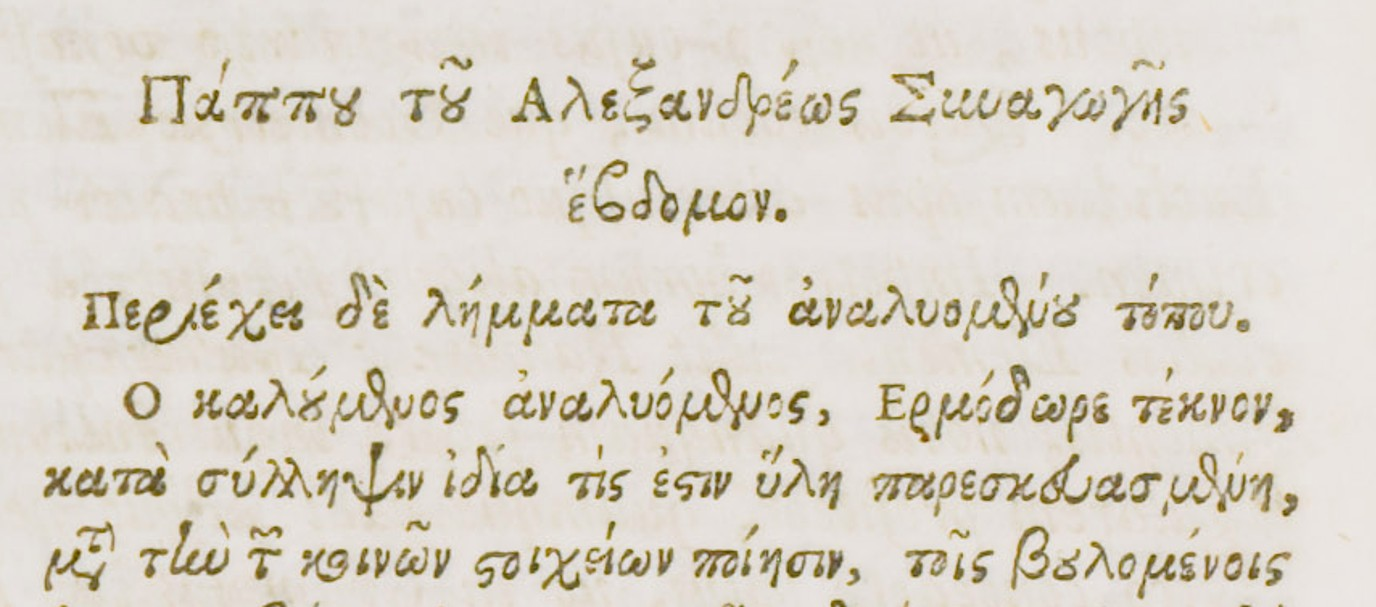
\includegraphics[scale=0.3]{greek_text_with_ligatures} 
%\caption{Sample text for Greek ligatures (Euclid lat/gr, p.16)} 
%\label{picture greek ligatures} 
%\end{figure}

%\ref{picture greek ligatures})
Transcription in four versions (with standardised β instead of ϐ, which is U+03D0): The first version is the easiest to read, which may be an advantage even with automated post-processing. Also, it makes it easier to encode the accents, see below.

$\to$ The Times font in which this XeTeX document is set doesn't have stigma and the alternative beta, and the combination of spiritus asper/lenis and an accent looks weird on the screen (prints fine on the Konica printer). Use a different font? Times New Roman has stigma and alternative beta and could be used for these characters.

$\to$ Greek characters in monospaced fonts: There are only a few monospaced fonts on the Mac, namely Courier, Courier New, Andale Mono, Monaco. Courier and Monaco don't have Greek characters. Andale Mono doesn't have complex characters such as alpha with accent and spiritus. Thus, only Courier New remains and can be seen below. Are we happy with it? The alternative would be a new monospaced font or a non-monospaced font such as Times/Times New Roman or Minion Pro.

\begin{typeGreek}
\begin{tabular}{l}
Πάππ(ου) τ(οῦ) Αλεξαν(δρ)έως Σ(υν)α(γω)(γῆ)ς \\ 
ἓβ(δο)(μο)ν. \\ 
Πε(ρι)έχ(ει) δὲ λήμμα(τα) τ(οῦ) ἀναλυο(μέν)(ου) (τό)(πο)υ. \\ 
Ο καλ(ού)(μεν)ος ἀναλυό(μεν)ος, Ερμόδωρε τέκνον, \\ 
κα(τὰ) σύ(λλ)η(ψι)ν ἰ(δί)α (τί)ς ἐ(στι)ν ὓλη (πα)ρε(σκ)[ευ]ασ(μέν)η, \\{}
[μετὰ] [τὴν] [τῶν] (κο)ινῶν (στο)ιχ(εί)ων (πο)ίη(σι)ν, (το)ῖς β(ου)λομένοις \\ 
\end{tabular}
\end{typeGreek}

(Last word: Either the alternative beta is not used at the beginning of the word or this is an alternative version of the capital beta; my guess is the former. Note that μέν is \emph{not} ligated here. The ου ligature is printed badly.)

\begin{typeGreek}
\begin{tabular}{l}
Πάππ<01> τ<01> Αλεξαν<07>έως Σ<23>α<04><03>ς \\ 
ἓβ<06><13>ν. \\ 
Πε<09>έχ<10> δὲ λήμμα<20> τ<01> ἀναλυο<02><01> <22><15>υ. \\ 
Ο καλ<01><02>ος ἀναλυό<02>ος, Ερμόδωρε τέκνον, \\ 
κα<20> σύ<12>η<24>ν ἰ<05>α <21>ς ἐ<18>ν ὓλη <14>ρε<16><25>ασ<02>η, \\ 
<26> <27> <28>  <11>ινῶν <19>ιχ<10>ων <15>ίη<17>ν, <22>ῖς β<01>λομένοις \\ 
\end{tabular}
\end{typeGreek}

\begin{typeGreek}
\begin{tabular}{l}
Πάππ(01) τ(01) Αλεξαν(07)έως Σ(23)α(04)(03)ς \\ 
ἓβ(06)(13)ν. \\ 
Πε(09)έχ(10) δὲ λήμμα(20) τ(01) ἀναλυο(02)(01) (22)(15)υ. \\ 
Ο καλ(01)(02)ος ἀναλυό(02)ος, Ερμόδωρε τέκνον, \\ 
κα(20) σύ(12)η(24)ν ἰ(05)α (21)ς ἐ(18)ν ὓλη (14)ρε(16)(25)ασ(02)η, \\ 
(26) (27) (28)  (11)ινῶν (19)ιχ(10)ων (15)ίη(17)ν, (22)ῖς β(01)λομένοις \\ 
\end{tabular}
\end{typeGreek}

\begin{typeGreek}
\begin{tabular}{l}
Πάππ01 τ01 Αλεξαν07έως Σ23α0403ς \\ 
ἓβ0613ν. \\ 
Πε09έχ10 δὲ λήμμα20 τ01 ἀναλυο0201 2215υ. \\ 
Ο καλ0102ος ἀναλυό02ος, Ερμόδωρε τέκνον, \\ 
κα20 σύ12η24ν ἰ05α 21ς ἐ18ν ὓλη 14ρε1625ασ02η, \\ 
26 27 28  11ινῶν 19ιχ10ων 15ίη17ν, 22ῖς β01λομένοις \\ 
\end{tabular}
\end{typeGreek}

The first version makes it easier to encode the accents. Alternative: 

\begin{typeGreek}
\begin{tabular}{l}
Πάππ<01> τ<01\textasciitilde> Αλεξαν<07>έως Σ<23>α<04><03\textasciitilde>ς \\ 
ἓβ<06><13>ν. \\ 
Πε<09>έχ<10> δὲ λήμμα<20> τ<01\textasciitilde> ἀναλυο<02´><01> <22´><15>υ. \\ 
Ο καλ<01´><02>ος ἀναλυό<02>ος, Ερμόδωρε τέκνον, \\ 
κα<20`> σύ<12>η<24>ν ἰ<05´>α <21´>ς ἐ<18>ν ὓλη <14>ρε<16><25>ασ<02´>η, \\ 
<26`> <27`> <28\textasciitilde>  <11>ινῶν <19>ιχ<10´>ων <15>ίη<17>ν, <22>ῖς β<01>λομένοις \\ 
\end{tabular}
\end{typeGreek}

Stigma-ligatures: (στι), or encode as (ςι), i.e. end-sigma and iota, and disambiguate later, or with proper stigma character U+03DB, i.e. (ϛι)? Probably (στι), because they will have to look it up anyway. Tilde or circumflex: The circumflex in the book looks like a modern tilde. Encode as circumflex anyway? (My Greek textbooks used the tilde, but it was called circumflex.)

The same text in Beta Code, with additional < and > for ligatures (probably a bad choice as there are possible collisions with milestone tags, e.g. <ti/>), capital and small letters rather than capital letters with and without an asterisk, comma (rather than apostrophe as in an ancient version of  Beta Code) to denote comma in the Greek text. Also, I would find it more natural to type the diacritics before rather than after the character, just as á is typed as ´a. Alternative for s1 and s2: Always type s and use disambiguation rules.

For Beta Code: It may be easier to type if one is familiar with the Latin alphabet. Against Beta Code: If the typists use a keyboard with Greek letters, even if they don't know the Greek language, it may help that they can immediately compare the shape of the letter in the book and in the typed text. The Thesaurus Linguae Graecae (TLG) uses Beta Code even though they have heard of Unicode 5.1, so they might have reasons? The main reason seems to be backwards compatibility, however. Is that an argument for us? (Even if the Chinese typists use Beta Code, our xml files will use Unicode.) By the way, the TLG's 2004 revision of Beta Code includes many unusual characters such as idiosyncratic abbreviations of ειναι (symbol \#1515), but no ligatures apart from ae etc.

\begin{type}\small
\begin{tabular}{l}
Pa/pp<ou> t<ou=> Alecan<dr>e/ws2 S<un>a<gw><gh=>s2 \\
e(b<do><mo>n. \\
Pe<ri>e/x<ei> de\textbackslash lh/mma<ta> t<ou=> a)naluo<me/n>ou <to/><po>u. \\
O kal<ou/><men>os2 a)naluo/<men>os2, Ermo/dwre te/knon, \\
ka<ta\textbackslash> s1u/<ll>h<yi>n i)<di/>a <ti/>s2 e)<s1ti>n u(lh <pa>re<s1k><eu>as<me/n>h, \\
<meta\textbackslash> <thn\textbackslash> <tw=n> <ko>inw=n <s1to>ix<ei/>wn <po>i/h<s1i>n, <to>i=s1 b<ou>lome/nois1 \\
\end{tabular}
\end{type}



Rule for vertical accents as in (τί)ς? 


\section{Book-specific Specifications}

\subsection{A Scheme for Book-specific Specifications}

\subsection{An Example}

